\documentclass[conference]{IEEEtran}

\usepackage{cite}
\usepackage{amsmath,amssymb,amsfonts}
\usepackage{graphicx}
\graphicspath{{../figures/}}
\usepackage{algorithm}
\usepackage{algpseudocode}
\usepackage{textcomp}
\usepackage{xcolor}
\usepackage{placeins}
\usepackage{booktabs}
\usepackage{url}
\usepackage[hidelinks]{hyperref}

\def\BibTeX{{\rm B\kern-.05em{\sc i\kern-.025em b}\kern-.08em
    T\kern-.1667em\lower.7ex\hbox{E}\kern-.125emX}}

\begin{document}

\title{Design of a Multimodal Pipeline for Accessibility in E-Learning Content}

\author{\IEEEauthorblockN{1\textsuperscript{st} Askar Nurym}
\IEEEauthorblockN{2\textsuperscript{nd} Zhukabayeva T. K.}
\IEEEauthorblockA{\textit{School of Software Engineering} \\
\textit{Astana IT University}\\
Astana, Kazakhstan \\
255453@astanait.edu.kz \\
t.zhukabayeva@astanait.edu.kz}
}

\maketitle

\begin{abstract}
The online learning format and educational videos are now deeply integrated into higher education and professional learning, but many platforms still leave captions, navigation and access to visual context as separate or incomplete features. This paper presents a prototype multimodal pipeline for processing source video into reusable artifacts: word-aligned captions, scene-indexed visual descriptions, summaries and chapter markers. The prototype player exposes keyboard-first controls, Accessible Rich Internet Applications (ARIA) semantics, configurable text presentation and word-level highlighting, but these are treated as design affordances rather than proof of user-level benefit. A bilingual corpus evaluation was conducted on 24 instructional videos (12 English, 12 Russian; 3.29 h total) using an automatic speech recognition (ASR)-only baseline (B0) and full multimodal configuration (B1). B1 stayed below real-time factor (RTF)=1.0 for every video, with mean RTF=0.433 and median RTF=0.424, compared with B0 mean RTF=0.193. ASR confidence is reported only as an internal diagnostic (mean 0.942). The 91.7\% 15-second scene coverage result describes temporal proximity to scene anchors, not description quality or accessibility impact. Results support prototype-stage engineering feasibility under resource and hosted-service constraints, while reference-based transcription error rates, qualitative description evaluation and user studies remain future work.

\end{abstract}

\begin{IEEEkeywords}
accessibility; e-learning; educational video; multimodal pipeline; automatic speech recognition; captioning; audio description; cognitive load
\end{IEEEkeywords}

\section{Introduction}
In higher education and professional growth, the video-centric format of education became dominant, but despite that, pre-recorded lessons and screen-captured records remain unfairly accessible across student groups. Studies show that captions, playback control, and navigational structure advance accessibility and support learning in video-based education environments \cite{Gernsbacher2015,Mayer2020,Horlin2024}. This prototype therefore, targets synchronized captions, scene-linked descriptions, and structured navigation within a single playback workflow.

Existing practice often treats these needs as separate product features. To solve that problem, the proposed work frames accessibility as an end-to-end pipeline problem: one processing flow should produce synchronized artifacts that can be reused by the playback layer and downstream tools. This framing is especially relevant under constrained deployment settings that have compute and application programming interface (API) quotas. Implementation complexity is a practical limitation. Prior work on automatic adaptation of open educational resources (OER) proposes a methodology for improving accessibility of existing educational content through AI-supported adaptation and accessibility metadata for search and reuse \cite{IngavelezGuerra2022}.

The research question is: Can a resource-constrained multimodal pipeline generate reusable accessibility-oriented artifacts for educational video with practical processing latency?

Contributions of research:
\begin{enumerate}
\item Implementation of a unified multimodal pipeline that simultaneously generates captions with word-level alignment and scene-indexed visual descriptions and structured summary.
\item Development of adaptive scene indexing that ensures complete coverage of content even with little difference between scenes, without predefining a fixed number of scenes.
\item Design of a system with an efficient on-demand scene audio-description mechanism, caching to reduce latency in case of repetitive local playbacks after the first request, support of accessibility for people with attention deficit hyperactivity disorder (ADHD) and dyslexia through fonts and captioning features.
\item Benchmarking on a balanced and normalized set of 24 educational videos in English and Russian languages.
\end{enumerate}

\section{Related Work}
\subsection{Captions and Learning Accessibility}
Caption benefits are not limited to impaired individuals; observations in the latest studies report benefits' extent beyond impaired learners for attention holding, comprehension of material, and recall \cite{Gernsbacher2015}. In educational environments, automated subtitles can be utilized under realistic conditions, but caption quality also depends on temporal alignment and segmentation precision \cite{Malakul2023}. This claim is supplemented by research of partial and fully synchronized captions; transcript quality alone is insufficient without temporal alignment \cite{Mirzaei2018}. W3C media-accessibility guidance also requires synchronized captions, content descriptions, playback control, and navigation \cite{W3CMediaReqs}. \textbf{Gap:} Inspection of most modern solutions shows isolated implementation of captions rather than integrated artifacts with multimodal support.

\subsection{Cognitive Load and Neurodiversity in Video Learning}
Instructional video effectiveness is defined by factors like pacing, signaling and learner control. Challenges related to media quality in online video lectures, including pace and speech intelligibility, directly affect the learning process \cite{Lange2020}. Measuring cognitive load of students during educational videos is dependent on context and difficult to reflect by a single metric \cite{Kruger2016}, and recent neurodiversity-focused researches highlight challenges related to transcription errors and limited playback/navigation control can create additional barriers for neurodivergent learners \cite{LeCunff2024,Horlin2024}. \textbf{Gap:} literatures motivates control and structure as learning supports, but it does not address how such supports can be generated automatically as reusable artifacts from raw educational video in a single processing pass.

\subsection{Automatic Speech Recognition and Timestamping}
Modern automatic speech recognition (ASR) systems have accomplished practical utility through deep-learning pipelines \cite{Malik2020} and large-scale weakly supervised models such as Whisper \cite{Radford2022}. Augmented methods such as WhisperX and CrisperWhisper target timestamp precision through forced alignment and attention-based refinement \cite{Bain2023,Wagner2024}. In the current prototype, ASR and timestamping mainly serve the caption artifact layer: they provide synchronized text that the player and downstream pipeline layers can reuse.

\subsection{Visual Accessibility and Audio Description}
Prior work on scene-description authoring offers quality evaluation of descriptions by descriptiveness, objectivity, succinctness, sufficiency, accuracy, referability, and clarity \cite{Natalie2021}. In this prototype, scene-linked descriptions are exposed as optional on-demand spoken output within the same processing pipeline rather than pre-rendered into the source media. The focus of the present study is systems integration and timing behavior, not a user-study evaluation of description quality.

\section{System Design}
\subsection{Pipeline Architecture and Artifacts}
The proposed system follows a \emph{Hybrid Multimodal Architecture}, which calls a remote multimodal large language model (LLM) for cognitively intensive tasks while utilizing deterministic algorithms for high-throughput media processing. To enhance performance on consumer-grade hardware, the acoustic (ASR) and visual (scene detection) branches execute concurrently. Given an input video, the system emits three artifact groups:
\begin{itemize}
\item \textbf{Subtitle artifacts} $A_{sub}$: word-level timestamps, segment timeline, and Web Video Text Tracks (WebVTT) export.
\item \textbf{Scene artifacts} $A_{scene}$: time-indexed visual scenes with text-aware natural-language descriptions.
\item \textbf{Structure artifacts} $A_{sum}$: summary points and chapter markers derived from scene descriptions.
\end{itemize}

\begin{figure*}[!t]
\centering
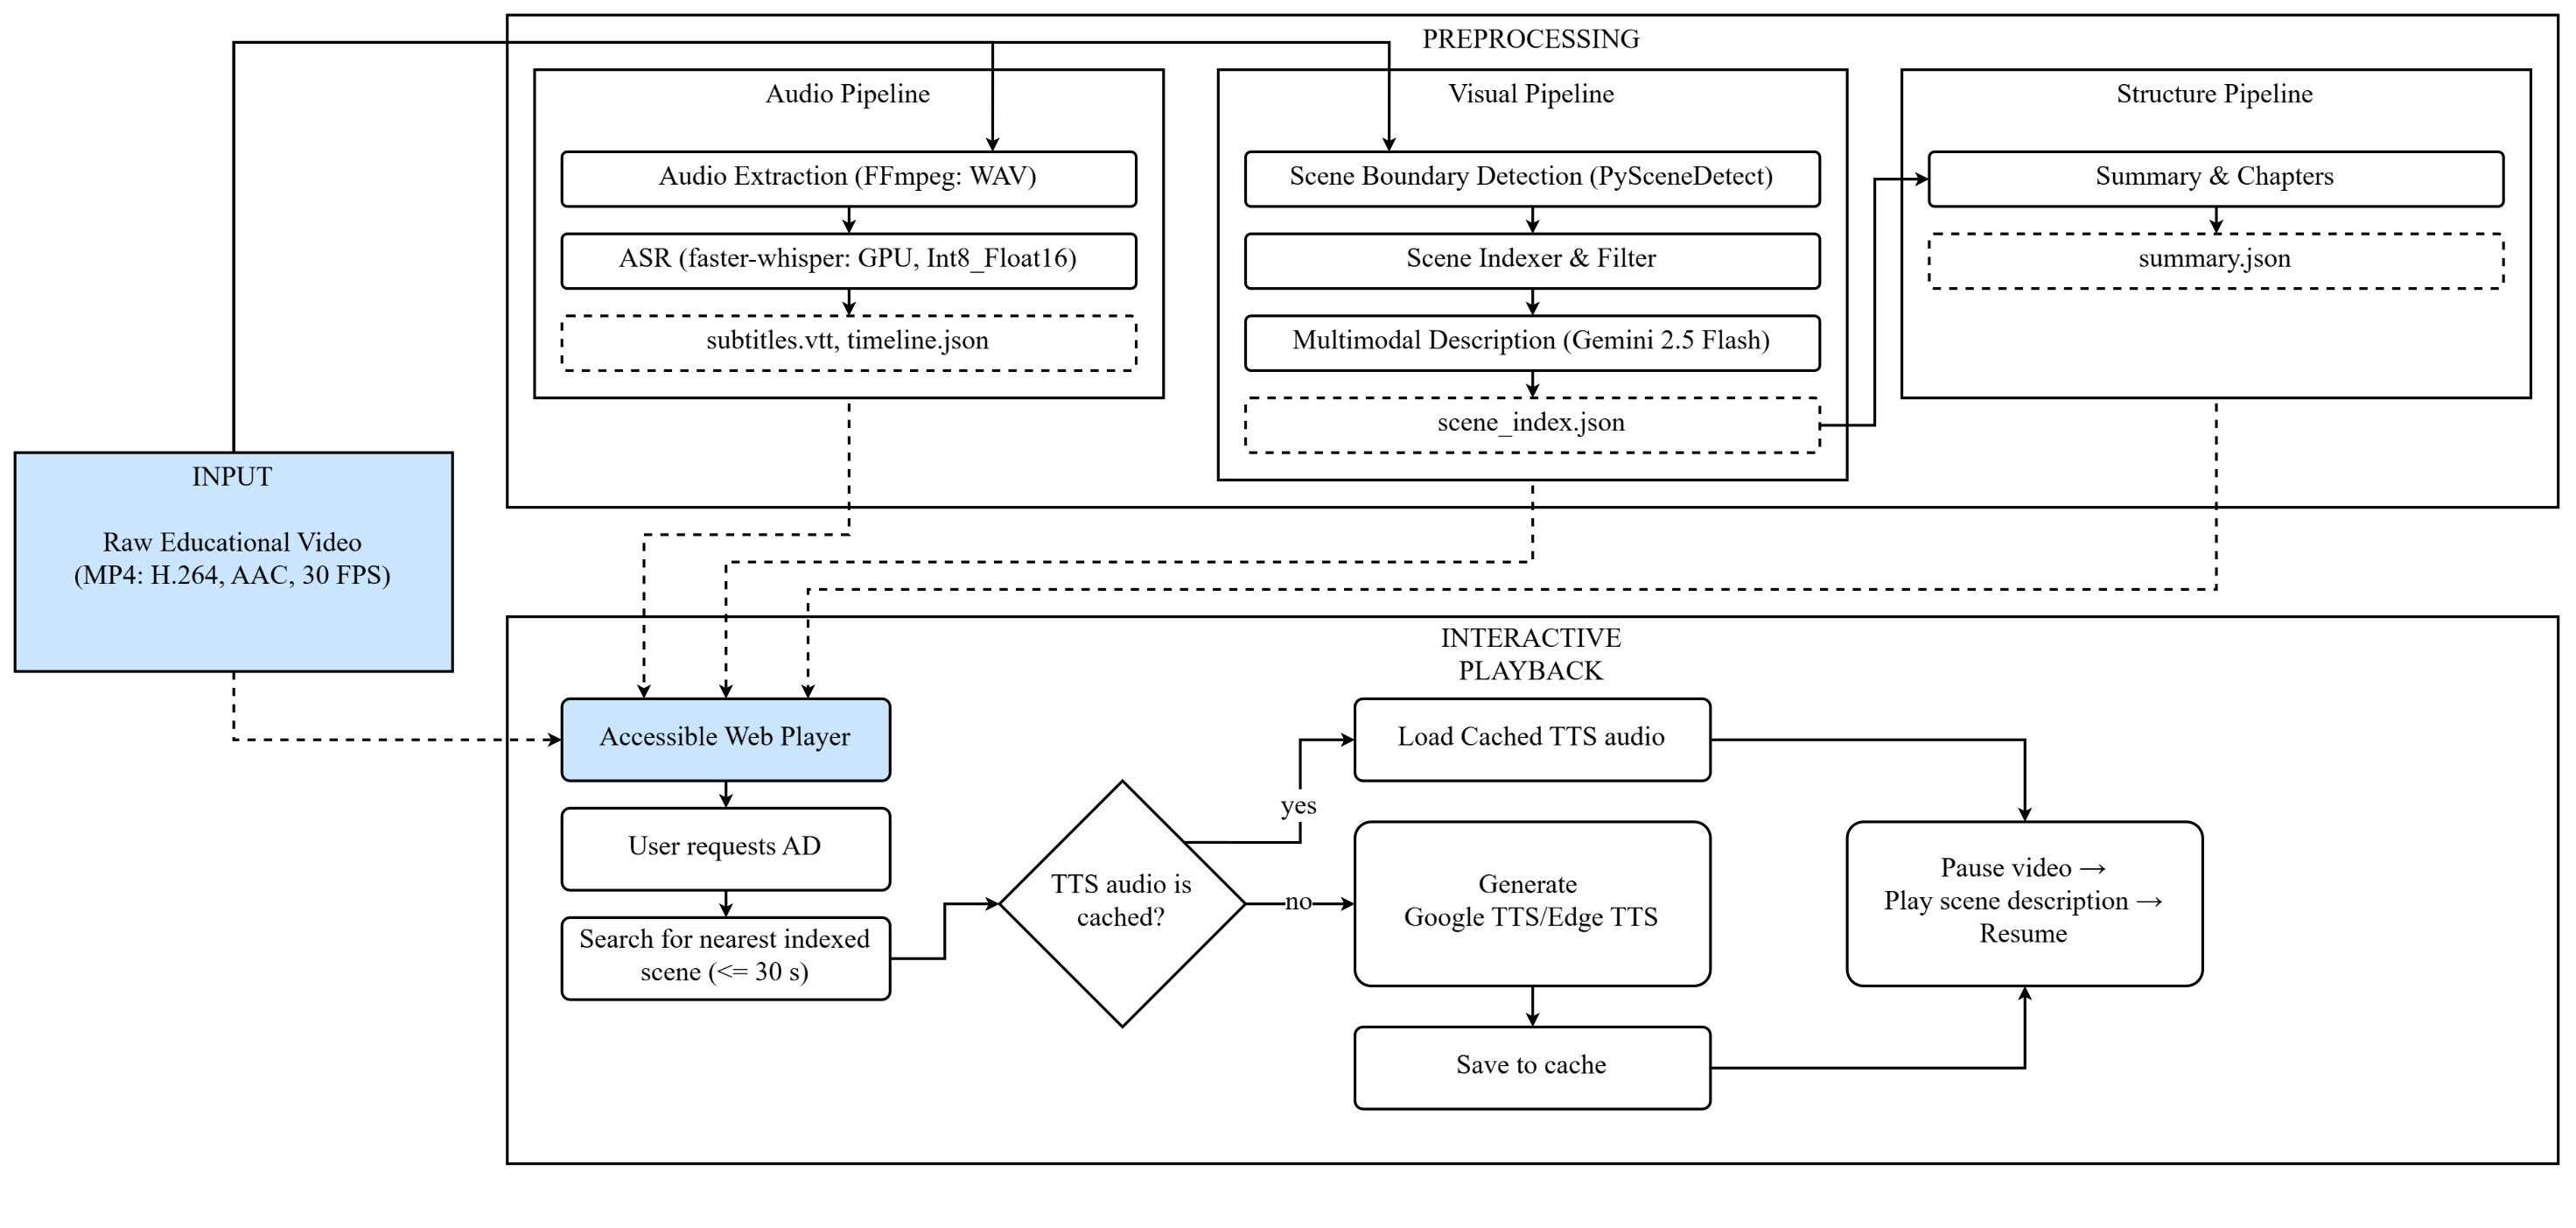
\includegraphics[width=0.95\textwidth]{fig_pipeline_arch.drawio.png}
\caption{Unified accessibility pipeline architecture. Offline preprocessing generates reusable artifacts; during playback, audio description is requested on demand and cached for subsequent calls.}
\label{fig:architecture}
\end{figure*}

\subsection{Interaction Layer and Artifact Rendering}
To implement karaoke highlighting we used a midpoint-based word grouper, which is intended to provide more stable word choice in the algorithm, avoiding temporal overlapping. Although in the evaluated corpus we have not detected any overlapping errors across adjacent words, we do not claim this to be fair for every other case.

Native HTML5 \texttt{<track>} elements do not fully satisfy the requirements selected for prototype player features such as granular, stateful word-by-word highlighting, including current, previous and upcoming states, and for this reason, we have implemented a custom web player subtitle renderer with user customizable font and contrast settings.

Audio description is played via on-demand mechanism reflected in Algorithm~\ref{alg:ad}: Player looks for the nearest indexed scene within 30 second threshold, then returns cached audio or calls a text-to-speech (TTS) function to synthesize speech from stored description and caches audio for later usage, then pauses the generated audio description and resumes original video playback.

\begin{algorithm}[!t]
\caption{On-Demand Audio Description Resolution}
\label{alg:ad}
\begin{algorithmic}[1]
\Require $T_{\text{req}}$ (current playback time in seconds)
\Require $I_{\text{scene}}$ (array of indexed scenes)
\Require $L_{\text{req}}$ (requested speech language)
\State $S_{\text{nearest}} \gets \text{select\_nearest}(I_{\text{scene}}, T_{\text{req}})$
\If{$|S_{\text{nearest}}.time - T_{\text{req}}| > 30.0$}
    \State \Return \text{Error (No scene nearby)}
\EndIf
\State $CacheKey \gets (S_{\text{nearest}}.id, L_{\text{req}})$
\If{\text{exists}($CacheKey$)}
    \State $Audio \gets \text{read\_cache}(CacheKey)$
\Else
    \If{\text{google\_tts\_available}()}
        \State $Audio \gets \text{synthesize\_preferred}(S_{\text{nearest}}.desc, L_{\text{req}})$
    \Else
        \State $Audio \gets \text{synthesize\_fallback}(S_{\text{nearest}}.desc, L_{\text{req}})$
    \EndIf
    \State $\text{write\_cache}(CacheKey, Audio)$
\EndIf
\State $\text{pause\_video}()$
\State $\text{play\_audio}(Audio)$
\State $\text{resume\_video}()$
\State \Return $Audio$
\end{algorithmic}
\end{algorithm}

\section{Methodology}
\subsection{Prototype Configuration}
Prototype implementation is currently focused on Russian and English languages support and instantiates the architecture described in Fig.~\ref{fig:architecture} with the following components:
\begin{enumerate}
\item \textbf{Transcribing:} system utilizes Whisper model optimized for \texttt{int8\_float16} compute type \cite{Radford2022}. This provides a balance between transcription accuracy and real-time factor (RTF).
\item \textbf{Visual Semantic Extraction:} Visual transitions are detected via an algorithm utilizing PySceneDetect library with pre-determined pixel difference threshold \cite{PySceneDetect}. In the next step, we utilize hosted \texttt{gemini-2.5-flash} multimodal model \cite{GeminiTeam2025} to generate a semantic description that encapsulates both textual and structural visual data from each identified scene.
\item \textbf{Adaptive Scene Indexing:} Because heuristic detection occasionally falls short on visually static content such as screencasts, we handle these low-variance scenarios by falling back to \emph{Adaptive Uniform Sampling}. This guarantees a baseline density of at least two descriptions per minute.
\end{enumerate}

\section{Technical Evaluation}
\subsection{Experimental Design and Corpus}
We evaluated the pipeline using a \emph{Bilingual Multimodal Corpus Benchmark} containing 24 educational videos (total duration of 197.61 minutes), 12 of which are in English, the other half is in Russian. For both languages we selected educational videos of various durations (short - 21.18 min, medium - 51.71 min, long - 124.73 min) and types of content (talking-head, slide-centric, screencast, and practical demo).

The videos were assembled from mixed educational sources and further normalized to 1280$\times$720 at 30 frames per second (FPS). The manifest preserves neither detailed source provenance nor license metadata, so the corpus should be treated as an internal engineering benchmark. Processing was conducted on a local workstation (AMD Ryzen 9 5900HX, NVIDIA RTX 3050 Notebook, 16 GB of RAM) to establish a baseline for consumer-grade deployability.

\begin{table}[t]
\caption{Corpus Composition}
\label{tab:corpus_comp}
\centering
\footnotesize
\setlength{\tabcolsep}{5pt}
\begin{tabular}{lccc}
\toprule
\textbf{Language} & \textbf{Short} & \textbf{Medium} & \textbf{Long} \\
\midrule
English & 4 & 4 & 4 \\
Russian & 4 & 4 & 4 \\
\bottomrule
\end{tabular}
\end{table}

Two configurations were compared:
\begin{itemize}
\item \textbf{B0 (ASR-only):} transcript and subtitle artifacts without visual branch.
\item \textbf{B1 (Full):} ASR + visual scene indexing + multimodal descriptions + summary/chapter generation.
\end{itemize}
Chosen configurations characterize pre-playback artifact generation. User-triggered text-to-speech call is not included in the full run process because of dependence on the network, the current user-grade test workstation is not enough to handle local multimodal LLM such as \texttt{gemini-2.5-flash}.

\begin{table}[t]
\caption{Key Experimental Parameters}
\label{tab:exp_params}
\centering
\footnotesize
\setlength{\tabcolsep}{4.5pt}
\begin{tabular}{ll}
\toprule
\textbf{Component} & \textbf{Setting} \\
\midrule
ASR model & faster-whisper medium \\
ASR compute type & int8\_float16 (GPU) \\
Scene detector & PySceneDetect ContentDetector \\
Scene threshold & 27 \\
Scene indexing & Adaptive density (no static cap) \\
Description stage & Hosted multimodal API \\
TTS (interactive path) & Google Cloud Neural TTS (edge-tts fallback) \\
Pipeline mode & On-demand audio description \\
\bottomrule
\end{tabular}
\end{table}

\subsection{Evaluation Metrics}
The study reports engineering proxy metrics, not direct measures of improved learning or accessibility effectiveness:
\begin{equation}
\text{low\_conf\_ratio} = \frac{w_{<0.5}}{w_{\text{all}}}
\end{equation}
\begin{equation}
\text{coverage}_{15s} = \frac{s_{\text{covered}}}{s_{\text{video}}}
\end{equation}
\begin{equation}
\text{RTF} = \frac{T_{\text{processing}}}{T_{\text{video}}}
\end{equation}
where RTF $< 1$ means preprocessing faster than the video duration.

For implementation, the denominators for both RTF and coverage are derived from the same effective video span: the end time of the generated timeline for each video. Thus, $T_{\text{video}}$ denotes the scalar duration used for RTF, while $s_{\text{video}}$ denotes the length of the evaluated timeline span used for coverage. This keeps B0/B1 denominators consistent for each video. In this definition, $T_{\text{processing}}$ includes pre-playback processing stages only; RTF is therefore interpreted as batch preprocessing throughput rather than end-to-end playback latency. ASR confidence is an internal diagnostic of Whisper model. Since no manual transcription accuracy checks, such as word error rate (WER) and character error rate (CER), were conducted, the metrics should not be interpreted as proof of transcription accuracy.

The metric $\text{coverage}_{15s}$ shows the proportion of evaluated video span covered by at least 1 scene anchor within a radius of 15 seconds. The 15-second radius was selected as half of the 30-second uniform grid used in the post hoc ablation. This metric does not indicate whether the generated description is sufficient or useful.

Additional diagnostics characterize alignment stability and visual indexing behavior:
\begin{equation}
\text{overlap\_ratio} = \frac{n_{\text{overlap}}}{\max(w_{\text{all}}-1,1)}
\end{equation}
\begin{equation}
\text{scene\_density} = \frac{n_{\text{scene}}}{T_{\text{video}}/60}
\end{equation}
\begin{equation}
\text{tail\_uncovered} = \max(0, T_{\text{video}} - t_{\text{last\_scene}})
\end{equation}
where $n_{\text{overlap}}$ is the number of overlapping adjacent word timestamps, and $t_{\text{last\_scene}}$ is the timestamp of the final indexed scene.

\subsection{Automation and Reproducibility}
All runs are conducted via a single driver script, which reads the corpus manifest and processes every video consecutively in B0 and B1 configurations; for single video processing, it applies a multithreaded pipeline scheme to reduce the total runtime. The driver saves pipeline output artifacts and computes summaries and metrics in machine-readable format, including baseline comparisons and a JavaScript Object Notation (JSON) report for further analysis. Tables and figures in this paper that are related to metrics are based on the 24-video corpus.

The system rejects runs before tables and summary metrics are generated by checking for non-positive runtimes, missing rows, and out-of-range coverage values. If there exist valid artifacts for the current set configuration, the driver will reuse them, which supports the cache-aware design of the pipeline. However, hosted model calls can return unexpectedly various results depending on model patches and network conditions.

\subsection{Post Hoc Scene Selection Ablation}
We conducted post-hoc scene selection ablation on a frozen evaluation snapshot. The same cached B1 scene timestamps were reused without rerunning the pipeline. We compared fixed caps of 10, 20 and 30 scenes with uniform 60 s and 30 s grids and recomputed the same within-15 s coverage metric. These comparisons are coverage-oriented diagnostics of scene-selection policy, not alternative semantic scene detection methods.

\subsection{Qualitative Case Selection}
In addition to obtained aggregate metrics, we selected four artifact sets from cached B1 outputs: the lowest coverage case, screencast reference, the densest practical demo and talking-head reference. These cases are used exclusively for surface-level checkups and do not serve to support semantic correctness or accessibility indicators for real users.

The selected cases are presented in the results section to link aggregate metrics with specific failure modes and design implications.

\FloatBarrier
\section{Results and Analysis}
\subsection{Aggregate Performance}
Table~\ref{tab:lang_overall} shows language-level and overall aggregates. The ASR component remains stable across languages (overall confidence mean 0.942 and low-confidence ratio mean 0.026). Baseline B0 is consistently fast (overall mean RTF 0.193), B1 adds slight overhead but remains practical (overall mean 0.433, median 0.424).

\begin{table}[t]
\caption{Aggregate Results by Language and Overall}
\label{tab:lang_overall}
\centering
\footnotesize
\setlength{\tabcolsep}{4.2pt}
\begin{tabular}{lcccccc}
\toprule
\textbf{Scope} & \textbf{N} & \textbf{B0} & \textbf{B1} & \textbf{B1} & \textbf{ASR} & \textbf{Cov.} \\
 &  & \textbf{RTF}\textsubscript{mean} & \textbf{RTF}\textsubscript{mean} & \textbf{RTF}\textsubscript{med} & \textbf{conf.} & \textbf{15s} \\
\midrule
EN & 12 & 0.158 & 0.369 & 0.353 & 0.948 & 91.58\% \\
RU & 12 & 0.228 & 0.497 & 0.504 & 0.937 & 91.82\% \\
Overall & 24 & 0.193 & 0.433 & 0.424 & 0.942 & 91.70\% \\
\bottomrule
\end{tabular}
\end{table}

\subsection{Baseline Overhead and Throughput Behavior}
Table~\ref{tab:duration_baseline} compares B0/B1 across short, medium and long videos. When comparing B0 mean RTF to B1 mean RTF, the highest overhead ratio is observed in the short videos set. Table~\ref{tab:stage_latency} shows the split absolute processing time (seconds) into the audio-only pipeline (B0) and visual semantic extraction overhead. The overhead increases with both scene count and video duration.

\begin{table}[t]
\caption{Stage-Level Latency Breakdown (Mean Seconds)}
\label{tab:stage_latency}
\centering
\footnotesize
\setlength{\tabcolsep}{5pt}
\begin{tabular}{lccc}
\toprule
\textbf{Duration} & \textbf{Audio Pipeline} & \textbf{Visual Overhead} & \textbf{Total (B1)} \\
\midrule
Short & 28.8 & 49.0 & 77.7 \\
Medium & 69.4 & 74.2 & 143.6 \\
Long & 191.6 & 193.6 & 385.3 \\
\bottomrule
\end{tabular}
\end{table}

\begin{table}[t]
\caption{Baseline Comparison by Duration Bucket}
\label{tab:duration_baseline}
\centering
\footnotesize
\setlength{\tabcolsep}{4.2pt}
\begin{tabular}{lcccc}
\toprule
\textbf{Duration} & \textbf{N} & \textbf{B0 RTF}\textsubscript{mean} & \textbf{B1 RTF}\textsubscript{mean} & \textbf{B1/B0} \\
\midrule
Short & 8 & 0.192 & 0.522 & 2.71$\times$ \\
Medium & 8 & 0.178 & 0.365 & 2.05$\times$ \\
Long & 8 & 0.208 & 0.414 & 1.99$\times$ \\
Overall & 24 & 0.193 & 0.433 & 2.25$\times$ \\
\bottomrule
\end{tabular}
\end{table}

Fig.~\ref{fig:rtf} visualizes B0 and B1 RTF across content types using boxplots. Full pipeline processing remains below real-time for all 24 videos in the corpus.

\begin{figure}[!t]
\centering
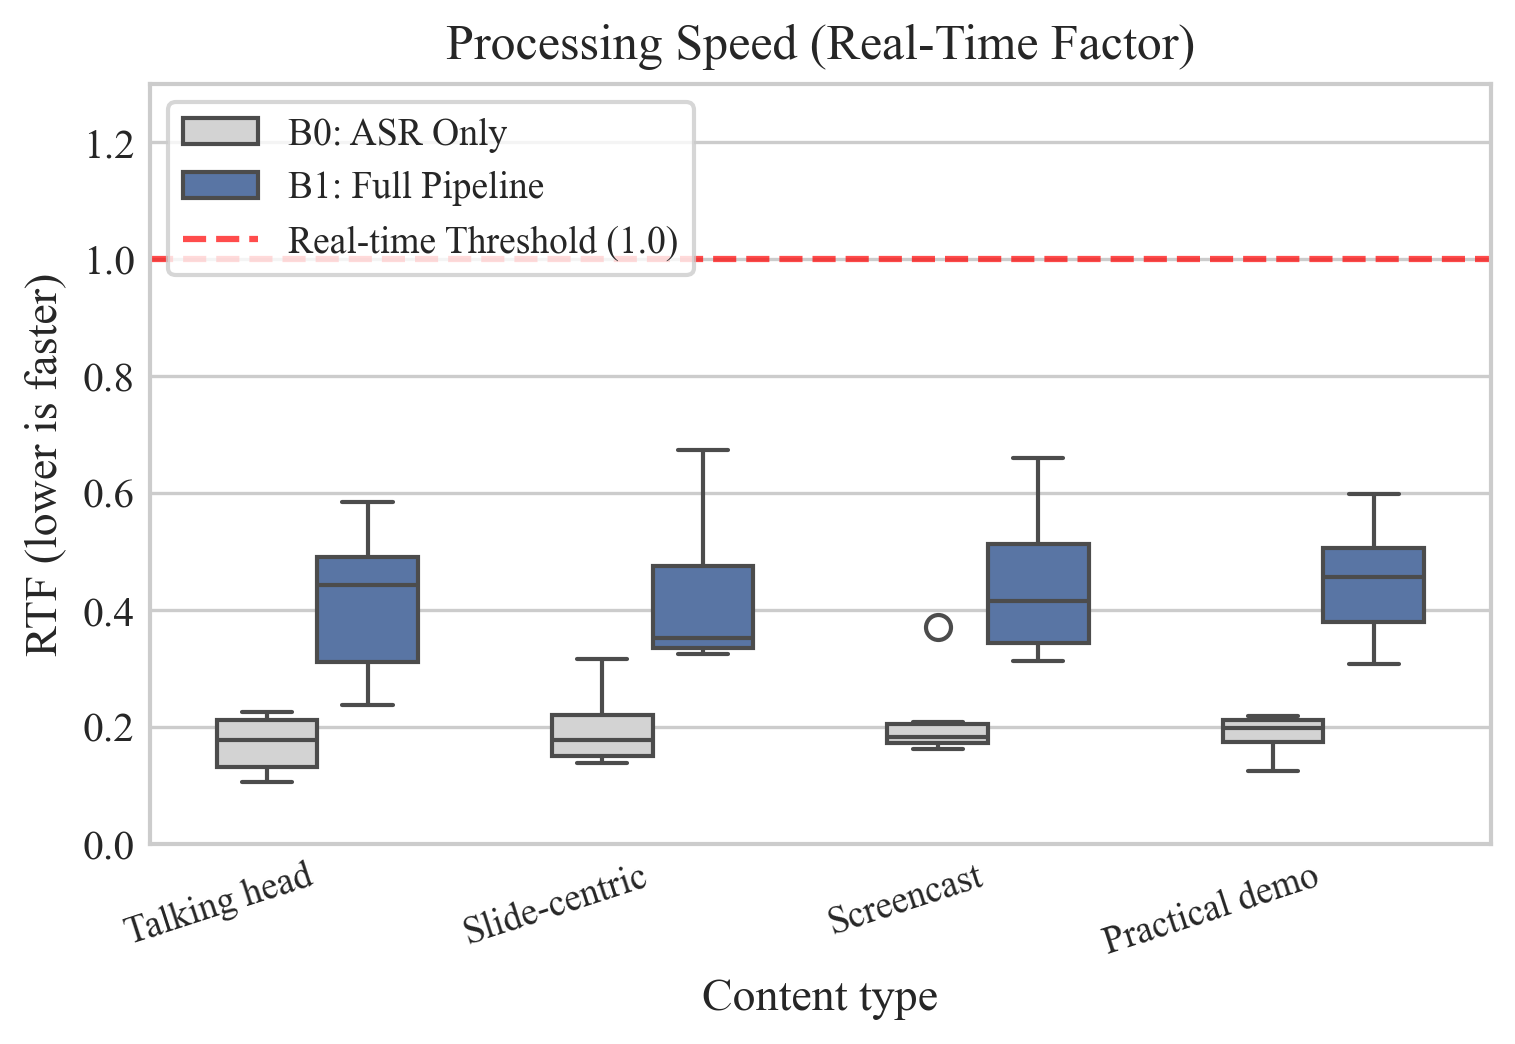
\includegraphics[width=\columnwidth]{fig_rtf_comparison.png}
\caption{Processing Speed (Real-Time Factor) across content types. The box spans the interquartile range (IQR), the horizontal line marks the median, and the whiskers denote the rest of the distribution up to $1.5 \times \text{IQR}$. A lower RTF indicates faster processing (the red dashed line represents real-time RTF=1.0).}
\label{fig:rtf}
\end{figure}

\subsection{Failure Cases and Practical Constraints}
Coverage variation is driven by visual characteristics. Low-variance screencasts remain a stress case for motion-based scene detection, so the pipeline applies fallback sampling when heuristic triggers are sparse. In the evaluated corpus, this kept screencast mean coverage at 94.58\%, while the overall mean coverage reached 91.7\%. Fig.~\ref{fig:coverage} shows the resulting content-type coverage distribution; the error bars summarize uncertainty within each six-video content-type group.

\begin{table}[t]
\caption{Content-Type Sensitivity (B1)}
\label{tab:content_sensitivity}
\centering
\footnotesize
\setlength{\tabcolsep}{4.2pt}
\begin{tabular}{lccccc}
\toprule
\textbf{Content type} & \textbf{N} & \textbf{B1 RTF} & \textbf{Cov. 15s} & \textbf{Scenes} & \textbf{Zero} \\
 &  & \textbf{mean} & \textbf{mean} & \textbf{mean} & \textbf{scene} \\
\midrule
Talking-head & 6 & 0.414 & 90.37\% & 29.83 & 0 \\
Slide-centric & 6 & 0.425 & 87.28\% & 33.67 & 0 \\
Screencast & 6 & 0.445 & 94.58\% & 39.00 & 0 \\
Practical demo & 6 & 0.449 & 94.55\% & 51.83 & 0 \\
\bottomrule
\end{tabular}
\end{table}

According to results presented in Table~\ref{tab:content_sensitivity}, screencast-type content appears to have the highest overall coverage when fallback sampling is used, while slide-centric content shows the lowest mean coverage, presumably because of rare slide transitions, which is typical for this type of content. Practical demos are the most saturated in terms of the mean detected scene count. All content types achieved coverage above 87\%.

\begin{table}[t]
\caption{Post Hoc Scene Selection Ablation}
\label{tab:scene_ablation}
\centering
\footnotesize
\setlength{\tabcolsep}{5pt}
\begin{tabular}{lcc}
\toprule
\textbf{Strategy} & \textbf{Scenes} & \textbf{Cov. 15s} \\
 & \textbf{mean} & \textbf{mean} \\
\midrule
Adaptive index & 38.58 & 91.69\% \\
Static cap 10 & 9.71 & 63.79\% \\
Static cap 20 & 16.62 & 80.25\% \\
Static cap 30 & 21.58 & 87.18\% \\
Uniform 60 s & 8.62 & 51.07\% \\
Uniform 30 s & 16.75 & 98.74\% \\
\bottomrule
\end{tabular}
\end{table}

Table~\ref{tab:scene_ablation} presents a trade-off comparison with ablation outcomes. Adaptive scene indexing shows the highest mean scene count (38.58 scenes) and the second-highest mean temporal coverage. Post-hoc caps of 10, 20 and 30 scenes reduced mean coverage 63.79\%, 80.25\%, and 87.18\%, respectively. The uniform 30 s interval achieved 98.74\% mean coverage because of a 15 s coverage radius, but this does not mean any quality improvements.

Selected cases illustrate why coverage should be interpreted with content type. The weakest case (\texttt{ru\_medium\_slide-centric}) reached 48.0\% coverage with 8 scenes and a 143.20 s maximum inter-scene interval, which fits rare-transition slide-centric content. In contrast, \texttt{en\_short\_screencast} reached 94.8\% with 12 scenes, and \texttt{en\_long\_practical\_demo} reached 100.0\% with 123 scenes and 429.17 s of B1 processing.

\begin{figure}[!t]
\centering
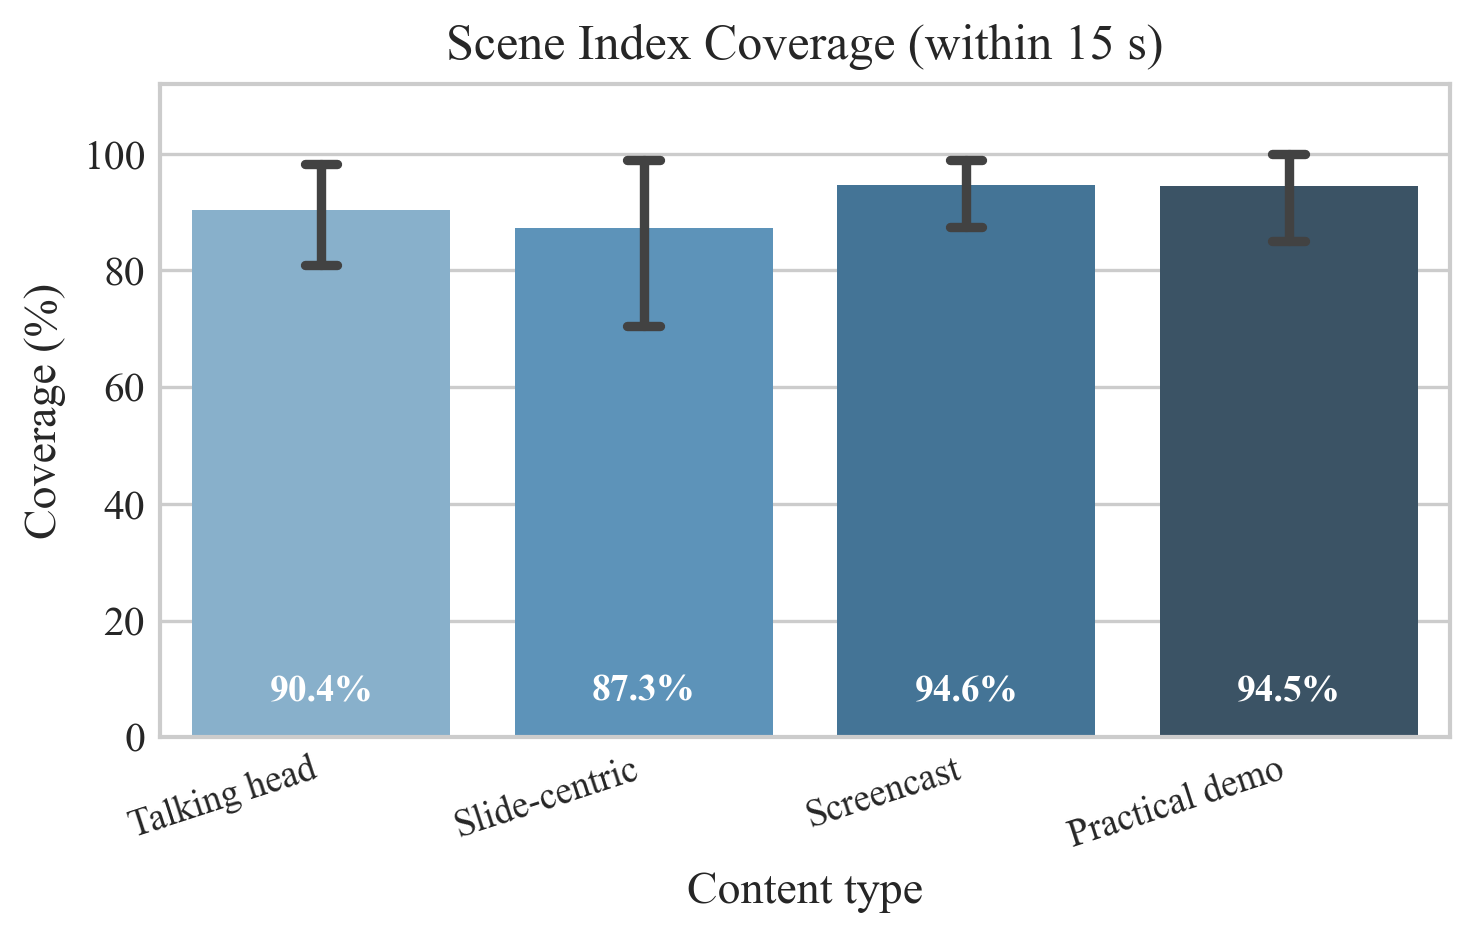
\includegraphics[width=\columnwidth]{fig_coverage.png}
\caption{Mean coverage within 15 s of indexed scenes by content type. Error bars show bootstrap 95\% confidence intervals computed from per-video values within each content-type group ($n=6$).}
\label{fig:coverage}
\end{figure}

\subsection{Interactive Latency and Speech Synthesis}
Separating text-to-speech (TTS) generation from corpus test runs avoids adding network-bound synthesis overhead to B1. A Google Cloud Neural TTS micro-benchmark on five sentence-level prompts showed median API latency of 2682.6~ms, while cached audio lookup took 0.06~ms. This spot-check excludes production network conditions, but still shows why request-level caching matters.

\section{Discussion}
\subsection{Interpretation of Baseline Overhead}
The B0/B1 ratio is an ablation-style system analysis. B0 captures a minimum subtitling path around Whisper ASR, while B1 adds visual transition indexing and visual context extraction. The 2.25 overhead ratio means that the full pipeline approximately doubles B0 processing time.

Duration results suggest amortization: initialization costs and API latencies affect short videos more strongly, while longer videos distribute these fixed costs across more content.

\subsection{Deployment Implications}


The main deployment dependencies remain hosted multimodal LLM and TTS services. Open-weight replacements are possible, but would require separate quality, runtime and hardware evaluation.

\section{Threats to Validity}
\textbf{External validity:} Balanced the 24-video corpus may not represent all possible real-world cases (heavy overlap speech, severe noise, extreme accents).

\textbf{Construct validity:} reported metrics are engineering proxies (timing quality, temporal coverage, throughput), not direct measures of learning gains or cognitive outcomes from human studies. The post-hoc ablation is coverage-oriented and does not compare semantic quality across scene-selection strategies. ASR confidence does not indicate actual transcription accuracy and cannot replace WER/CER validation.

\textbf{Internal validity:} the visual context extraction and on-demand TTS stages rely on hosted API calls, which introduces network, rate-limit and model-drift dependencies. Benefits were not evaluated with targeted user groups, so the prototype cannot claim direct user impact. We mitigate engineering risks through artifact persistence and explicit stage-aware reporting.

\section{Conclusion}
This paper presented a viable unified processing pipeline for generating reusable educational-video artifacts with multimodal accessibility support. The prototype employs ASR-based word-level captions, adaptive scene indexing, remote visual description generation, and TTS combined into one workflow without modifying the source content. The main contribution of this work is therefore proving engineering feasibility and artifact architecture, not user-level impact.
The bilingual evaluation corpus of 24 videos supports feasibility under the tested workstation and hosted-service conditions. The full B1 processing pipeline stayed below real-time for every evaluated video, with mean RTF=0.433 and median RTF=0.424, while B0 (ASR-only) baseline pipeline run showed mean RTF=0.193. Adaptive scene indexing reached 91.7\% mean temporal coverage within 15 seconds of an indexed scene.
Future work should move towards stronger validation of transcription and verification of positive impact for real target users. Transcripts need WER/CER or manual checking; scene descriptions need qualitative review for accuracy, sufficiency, and usefulness; the player experience needs to be evaluated by relevant user groups or accessibility experts. A larger test corpus with explicit source provenance and license metadata would make the benchmark more reproducible.

\bibliographystyle{IEEEtran}
\bibliography{references}

\end{document}
